%%%%%%%%%%%%%%%%%%%%%%%%%%%%%
%Since : 2019/04/03
%Update: 2020/04/23
% -*- coding: utf-8 -*-
%%%%%%%%%%%%%%%%%%%%%%%%%%%%%

\chapter{Excelによる統計処理2}
\setcounter{num_prac}{0}

\section{目的}

データ解析おいて重要なデータの可視化(グラフ化)の方法を学ぶ.

\section{グラフ}

データの特徴を視覚的に把握するためにグラフを用います.
代表的なグラフの一つが前回取り扱ったヒストグラムです.
ヒストグラム以外にも様々なグラフが存在します.
今回は,棒グラフ,折れ線グラフ,散布図を取り扱います.

\subsection{棒グラフ}

\paragraph{棒グラフとは}

棒グラフは値の大きさの比較に用いられます.
例えば,表\ref{tab:uriage}に示す商品の売上高をグラフ化すると図\ref{fig:bar}のようになります.
グラフにしたことで,それぞれの商品の売上の大小が視覚的に分かりやすくなります.
しかし,棒グラフは基本的に時間変化を把握するためには用いません.

\begin{figure}[htbp]
    \begin{minipage}{0.5\hsize}
        \centering
        \makeatletter
        \def\@captype{table}
        \makeatother
        \caption{}
        \begin{tabular}{|c|c|}
          \hline
          \multicolumn{2}{|c|}{4月の売上高}\\ \hline
          商品  & 売上高 (万円) \\ \hline
          商品A & 350 \\ \hline
          商品B & 120 \\ \hline
          商品C & 50 \\ \hline
          商品D & 250 \\ \hline
        \end{tabular}
        \label{tab:uriage}
    \end{minipage}
    \begin{minipage}{0.5\hsize}
        \centering
        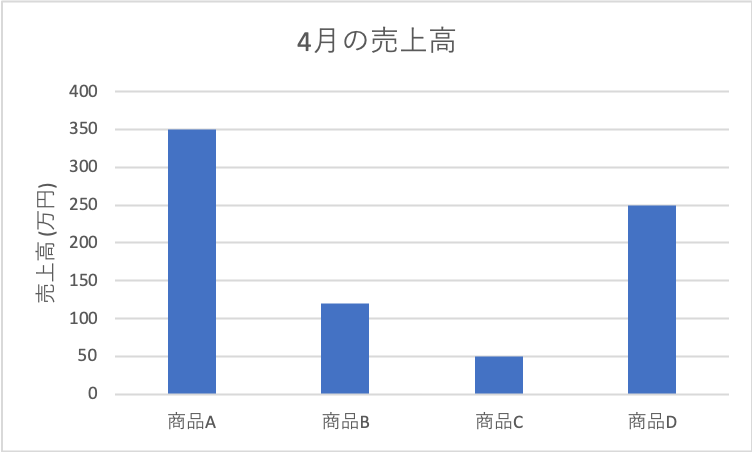
\includegraphics[width=6cm]{chap2/bar.png}
        \caption{棒グラフ}
        \label{fig:bar}
    \end{minipage}
\end{figure}

\paragraph{棒グラフの作成}

手順は前回のヒストグラムと同じです.表\ref{tab:uriage}に示すデータを棒グラフにしましょう.

\begin{enumerate}
    \item データを入力します.今回は図\ref{fig:bar1}のように入力してください.
    \item 棒グラフにしたいデータを図\ref{fig:bar1}のように選択します.
    \item リボンの挿入を押します.
    そして,リボンにある棒グラフアイコンを押し,図\ref{fig:select_barchart_hist}に示す棒グラフボタンを押します.
    そうすると,図\ref{fig:bar3}のような棒グラフができます.
    \item 出来上がったグラフには軸のラベルがありません.軸が何をあらわすか分かるようにラベルを付けます.
    \begin{enumerate}
        \item 軸にラベルを追加するには,軸を加えたいグラフをクリックし (グラフが選択された状態で),リボンのグラフのデザインをクリックします.
        \item そして,リボンのグラフ要素を追加をクリックします.
        \item 出てきたメニュー (図\ref{fig:bar_label}) の軸ラベル第1縦軸を選びます.
        そうすると,縦軸に``軸ラベル''というラベルが追加されます.
        \item ``軸ラベル''をクリックし選んだあと,更にクリックすると編集できるようになります.
        縦軸は``売上金額 (万円)''にしましょう\footnote{軸には単位を付けましょう.}.
        \item 必ずしもグラフにタイトル付ける必要はありませんが,今回はタイトルを付けます.
        ``グラフ タイトル''をクリックし選んだあと,更にクリックすると編集できるようになります.
        グラフタイトルを``4月の売上金額''にしましょう.そうすると図\ref{fig:bar}のようなグラフができます.
    \end{enumerate}
\end{enumerate}

\begin{figure}[tb]
    \begin{minipage}{0.5\hsize}
        \centering
        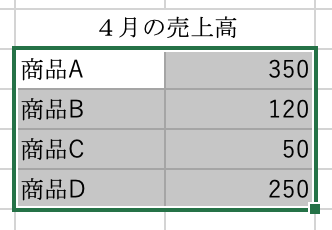
\includegraphics[width=4cm]{chap2/bar1.png}
        \caption{データを選択した状態}
        \label{fig:bar1}
    \end{minipage}
    \begin{minipage}{0.5\hsize}
        \centering
        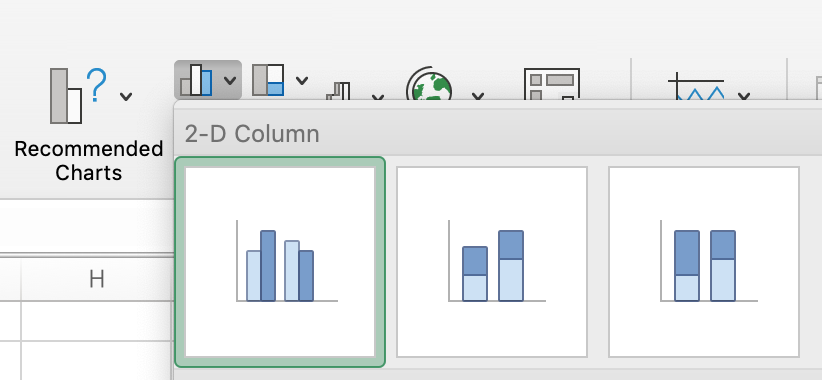
\includegraphics[width=6cm]{chap2/bar2.png}
        \caption{棒グラフを選択する}
        \label{fig:bar2}
    \end{minipage}
\end{figure}

\begin{figure}[tb]
    \begin{minipage}{0.5\hsize}
        \centering
        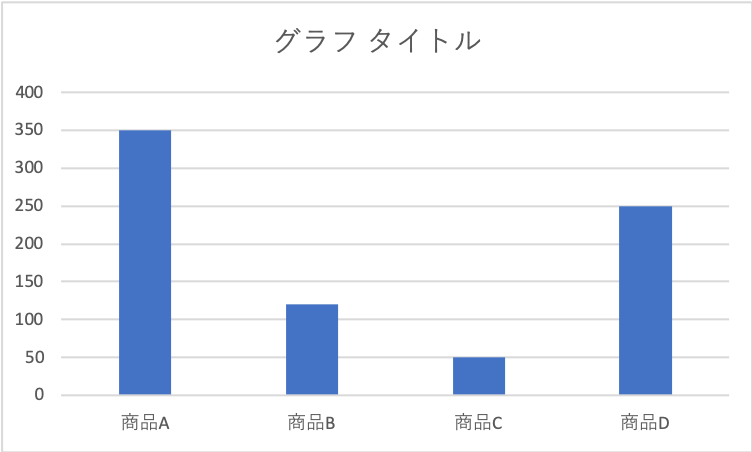
\includegraphics[width=6cm]{chap2/bar3.png}
        \caption{作成したグラフ}
        \label{fig:bar3}
    \end{minipage}
    \begin{minipage}{0.5\hsize}
        \centering
        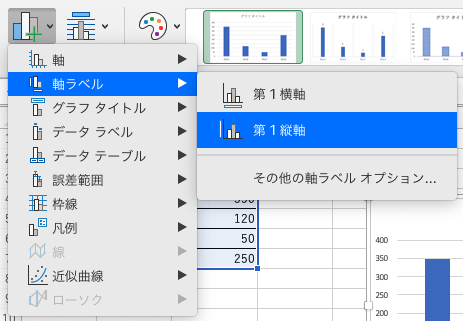
\includegraphics[width=6cm]{chap2/bar_label.png}
        \caption{軸ラベルを追加する}
        \label{fig:bar_label}
    \end{minipage}
\end{figure}


\subsection{折れ線グラフ}

\paragraph{折れ線グラフとは}

折れ線グラフは値の時間変化の把握のために用いられます.
例えば,表\ref{tab:uriage_suii}に示す商品の売上高の推移をグラフ化すると,図\ref{fig:line}のようになります.
商品の売上が時間とともに変化していることが,グラフ化することで視覚的に分かりやすくなります.
特に,商品Bと商品Cの売上がいつ,どのように逆転したのかグラフ化することでよく分かります.
ただし,大きさを比べる目的で折れ線グラフを使わないようにしましょう.

\begin{figure}[htbp]
    \begin{minipage}{0.5\hsize}
        \centering
        \makeatletter
        \def\@captype{table}
        \makeatother
        \caption{}
        \begin{tabular}{|c|c|c|}
          \hline
          \multicolumn{3}{|c|}{売上高(万円)}\\ \hline
          月& 商品B & 商品C \\ \hline
          4 &  120 & 50\\ \hline
          5 &  120 & 55\\ \hline
          6 &  110 & 75\\ \hline
          7 &  90  & 80\\ \hline
          8 &  100 & 110\\ \hline
          9 &  80  & 120\\ \hline
        \end{tabular}
        \label{tab:uriage_suii}
    \end{minipage}
    \begin{minipage}{0.5\hsize}
        \centering
        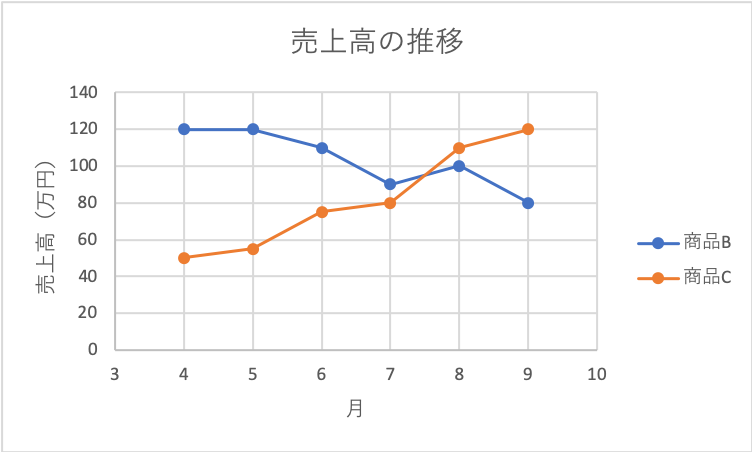
\includegraphics[width=6cm]{chap2/line.png}
        \caption{折れ線グラフ}
        \label{fig:line}
    \end{minipage}
\end{figure}

\paragraph{折れ線グラフの作成}

表\ref{tab:uriage_suii}に示すデータを折れ線グラフにします.横軸を月,縦軸を売上金額とします.

\begin{enumerate}
    \item データを入力します.今回は図\ref{fig:line_select_data}のように入力してください.
    \item 図\ref{fig:line_select_data}のように横軸のデータと縦軸のデータを選びます.
    値だけではなく商品名まで選択しました.
    そうするとグラフの線の説明(凡例)まで自動で入力されます
    \footnote{いつもうまくいくとは限りません.
      うまく凡例がつかなかったときは,値だけ選択してグラフをかきます.
      グラフを選択し,リボンのグラフのデザインを選び,グラフデータの選択をクリックします.
      そうするとウインドウが出てくるので,そのウインドウにある名前の欄に凡例を書き込みます.}.
    \item グラフの散布図の直線とマーカーを選びます
    \footnote{折れ線グラフを選んでもグラフはかけますが,軸の範囲が固定など面倒なことになります.今回は散布図にします.}.
    そうすると図\ref{fig:line1}のようなグラフがかけます.
    \item 凡例が下だと邪魔ですので右に移動させます.
    グラフを選択し,リボンのグラフのデザインをクリックします.
    グラフ要素の追加をクリックし,凡例にカーソルを移動させると,図\ref{fig:line_hanrei}のように凡例の場所を選ぶことができます.
    そうすると,図\ref{fig:line2}のようになります.
    \item 図\ref{fig:line2}を見れば分かりますが,線がグラフ全体に広がらず右上に偏っています.
    軸の値の範囲を変更して,線を全体に広げます.
    \begin{enumerate}
        \item 横軸をクリックし (選び),右クリックを押して出てくる軸の書式設定 (図\ref{fig:line_axis}) を選びます.
        \item ウインドウの右端に出てくる軸の書式設定 (図\ref{fig:line_range}) の最小値,最大値を変更します.
        今回は最小値を3.0,最大値を10.0とします.
        同様のやり方で,縦軸の最小値を40.0,最大値を130.0とします.
        そうすると図\ref{fig:line3}のようになります.
    \end{enumerate}
    \item 軸のラベルを追加します
    \begin{enumerate}
        \item 軸にラベルを追加するには,まず,軸を加えるグラフを選び,リボンのグラフのデザインをクリックします.
        \item リボンのグラフ要素を追加をクリックします.
        \item 出てきたメニュー (図\ref{fig:line_label}) の軸ラベル第1縦軸を選びます.
        そうすると,縦軸に``軸ラベル''というラベルが追加されます.
        \item ``軸ラベル''をクリックし選んだあと,更にクリックすると編集できるようになります.
        縦軸は``売上高 (万円)''にしましょう\footnote{軸には単位を付けましょう.}.同様の手順で横軸を``月''にしましょう.
        そうすると,図\ref{fig:line4}のようなグラフができます.
    \end{enumerate}
    \item 必ずしもグラフにタイトル付ける必要はありませんが,今回はタイトルを付けます.
    ``グラフ タイトル''をクリックし選んだあと,更にクリックすると編集できるようになります.
    その状態で,``売上高の推移''に変更しましょう.
    以上の操作で,図\ref{fig:line}のようなグラフになります.
\end{enumerate}

\begin{figure}[tb]
    \begin{minipage}{0.5\hsize}
        \centering
        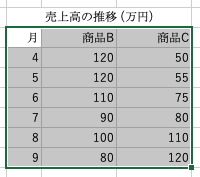
\includegraphics[width=5cm]{chap2/line_select_data.png}
        \caption{データの選択}
        \label{fig:line_select_data}
    \end{minipage}
    \begin{minipage}{0.5\hsize}
        \centering
        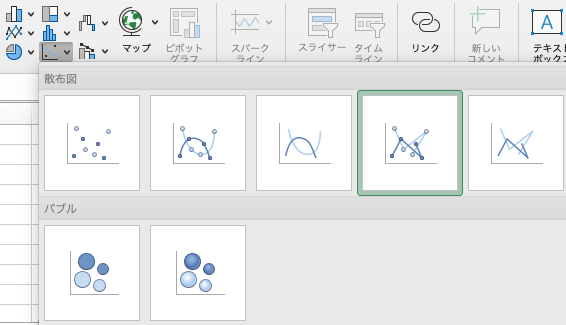
\includegraphics[width=6cm]{chap2/line_menu.png}
        \caption{散布図の直線とマーカーを選択する}
        \label{fig:line_menu}
    \end{minipage}
\end{figure}

\begin{figure}[tb]
    \begin{minipage}{0.5\hsize}
        \centering
        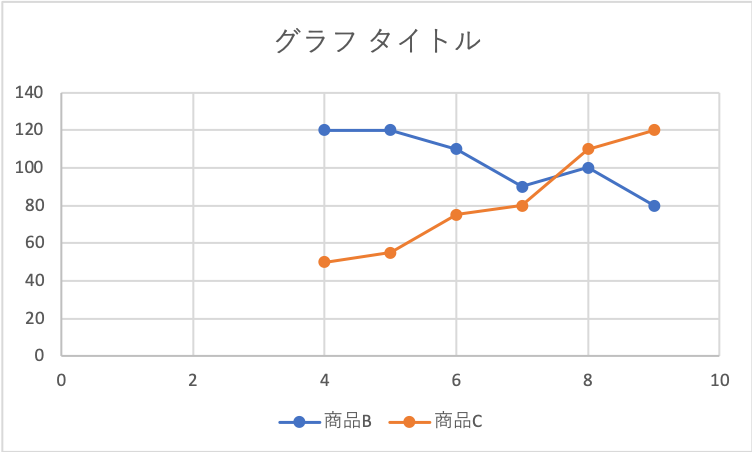
\includegraphics[width=6cm]{chap2/line1.png}
        \caption{作成されたグラフ1}
        \label{fig:line1}
    \end{minipage}
    \begin{minipage}{0.5\hsize}
        \centering
        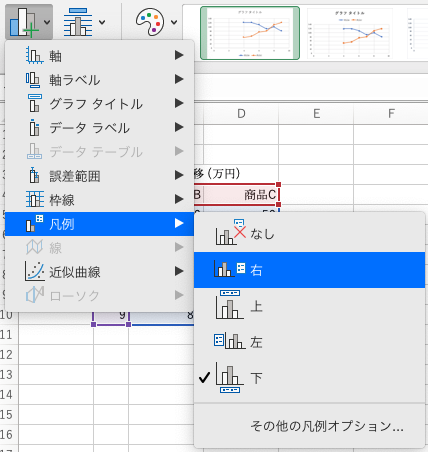
\includegraphics[width=6cm]{chap2/line_hanrei.png}
        \caption{凡例の位置}
        \label{fig:line_hanrei}
    \end{minipage}
\end{figure}

\begin{figure}[tb]
    \begin{minipage}{0.5\hsize}
        \centering
        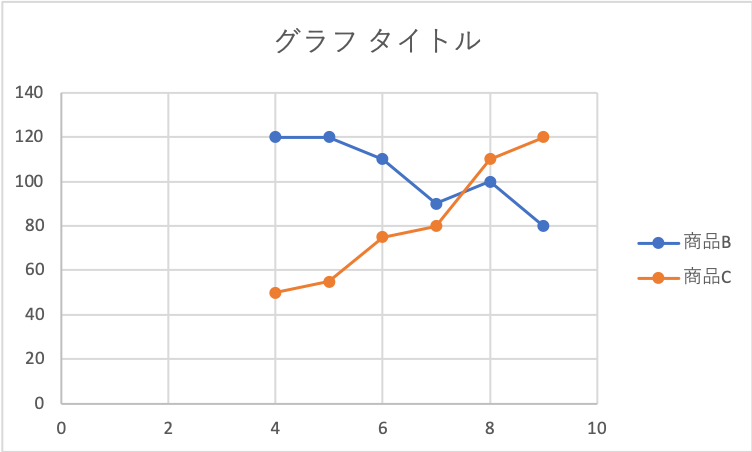
\includegraphics[width=6cm]{chap2/line2.png}
        \caption{作成されたグラフ2}
        \label{fig:line2}
    \end{minipage}
    \begin{minipage}{0.5\hsize}
        \centering
        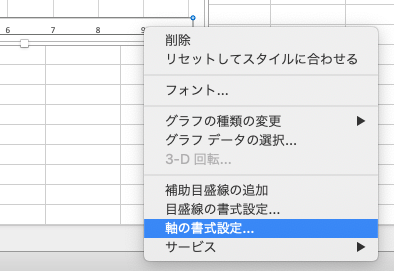
\includegraphics[width=6cm]{chap2/line_axis.png}
        \caption{軸の書式設定クリックする}
        \label{fig:line_axis}
    \end{minipage}
\end{figure}

\begin{figure}[tb]
    \begin{minipage}{0.5\hsize}
        \centering
        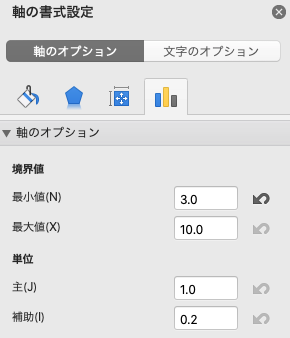
\includegraphics[width=4cm]{chap2/line_range.png}
        \caption{軸の範囲を変更}
        \label{fig:line_range}
    \end{minipage}
    \begin{minipage}{0.5\hsize}
        \centering
        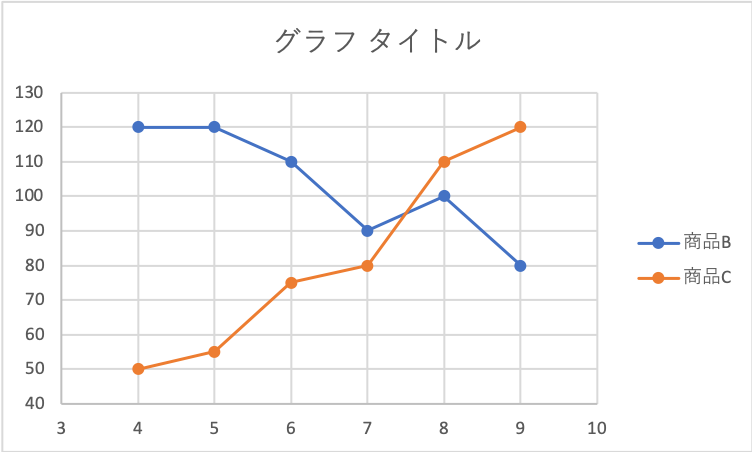
\includegraphics[width=6cm]{chap2/line3.png}
        \caption{作成されたグラフ3}
        \label{fig:line3}
    \end{minipage}
\end{figure}

\begin{figure}[tb]
    \begin{minipage}{0.5\hsize}
        \centering
        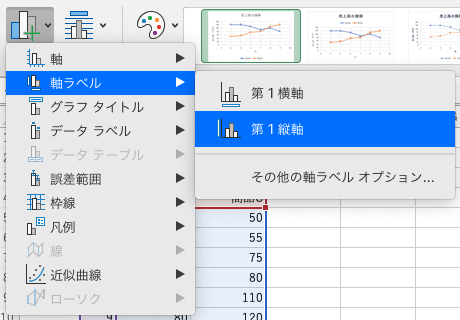
\includegraphics[width=4cm]{chap2/line_label.png}
        \caption{軸のラベルを追加}
        \label{fig:line_label}
    \end{minipage}
    \begin{minipage}{0.5\hsize}
        \centering
        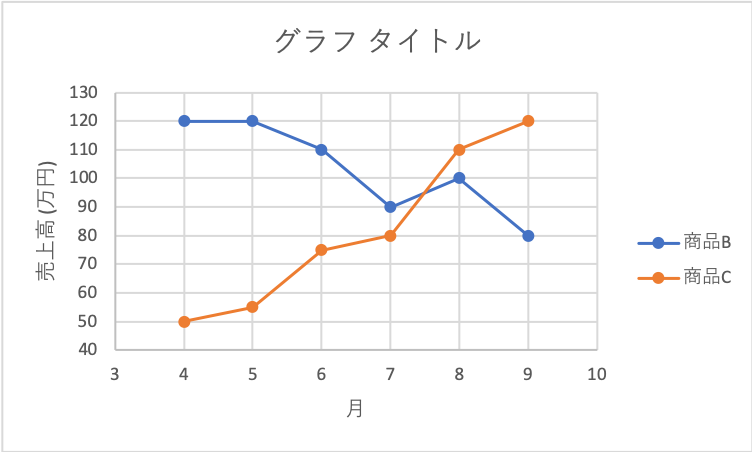
\includegraphics[width=6cm]{chap2/line4.png}
        \caption{作成されたグラフ4}
        \label{fig:line4}
    \end{minipage}
\end{figure}

\subsection{円グラフ}

前回,表\ref{tab:countif}から出身県ごとの人数を計算しました.では,各出身県出身者の人数の全体の割合がどの様になっているのか視覚的に分かりやすくするにはどうすればよいでしょうか.このようなときは,円グラフを用います.
円グラフは,円を扇型に分割し,その扇型に割当てられた割合の大きさに応じ扇型の角度を決めたものです.
扇型に割り当てられた割合をすべて足すと100\%になります.
逆に言えば,円一周で100\%にならなければなりません.
図\ref{fig:piechart}は表\ref{tab:countif}から作成した出身県の人数の割合を表す円グラフです.

\begin{figure}
\begin{minipage}{0.5\hsize}
    \centering
    \makeatletter
    \def\@captype{table}
    \makeatother
    \caption{データ}
    \begin{tabular}{|c|c|c|}
      \hline
      番号& 出身県\\ \hline
      1   & 石川  \\ \hline
      2   & 福井  \\ \hline
      3   & 富山  \\ \hline
      4   & 石川  \\ \hline
      5   & 岐阜  \\ \hline
      6   & 福井  \\ \hline
      7   & 石川  \\ \hline
      8   & 大阪  \\ \hline
      9   & 石川  \\ \hline
      10  & 富山  \\ \hline
    \end{tabular}
    \label{tab:countif}
\end{minipage}
\begin{minipage}{0.5\hsize}
    \centering
    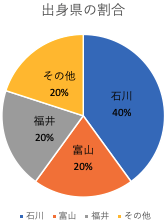
\includegraphics[width=6cm]{chap2/piechart.png}
    \caption{円グラフ}
    \label{fig:piechart}
\end{minipage}
\end{figure}


\paragraph{円グラフの作成}

表\ref{tab:countif}に示すデータから出身券の割合を円グラフにします.

\begin{enumerate}
    \item 前回行ったCOUNTIF,COUNTIFSの演習で作成したエクセルファイルを開きます.そのファイルにはすでに図\ref{fig:piechart_data}のように各県の出身者が計算されているはずです.
    \item 図\ref{fig:piechart_select_data}のように円グラフにしたい系列と値を選びます.
    \item リボンの挿入を押します.そしてグラフアイコンの中で円グラフを押すと図\ref{fig:piechart_menu}のように表示されます.その中で2D円の左端のものをクリックします.
    そうすると,図\ref{fig:piechart_plain}のようなグラフができます.
    \item この状態では,グラフに割合が入っていないなど味気ないですね.そこで次に,グラフに割合を表示させましょう.まず,グラフをクリックし,リボンのグラフのデザインをクリックします.そして,グラフ要素を追加をクリックし,マウスカーソルをデータラベルに移動させると,図\ref{fig:piechart_label_menu}のように表示されます.ここでは中央を選びます.そうすると,グラフが図\ref{fig:piechart_labeled}のようにグラフに人数が表示されます.
    \item 人数ではなく割合(パーセンテージ)に表示を変えます.変えるには,人数を選び右クリックをします.そうすると,図\ref{fig:piechart_select_label_option}のように表示されるので,それのデータラベルの書式設定をクリックします.そうすると,ウインドウの右端に図\ref{fig:piechart_label_option}が表示されます.図のように,分類名,パーセンテージにチェックを入れます.今回は,引き出し線はチェックしてもしなくても良いです.
    \item 最後に,タイトルを編集します.グラフ タイトルをダブルクリックし,出身県に変えます.そうすると,図\ref{fig:piechart}が完成します.
\end{enumerate}

\begin{figure}[tb]
    \begin{minipage}{0.5\hsize}
        \centering
        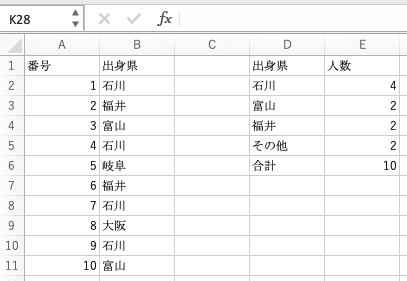
\includegraphics[width=5cm]{chap2/piechart_data.png}
        \caption{ファイルを開いた状態}
        \label{fig:piechart_data}
    \end{minipage}
    \begin{minipage}{0.5\hsize}
        \centering
        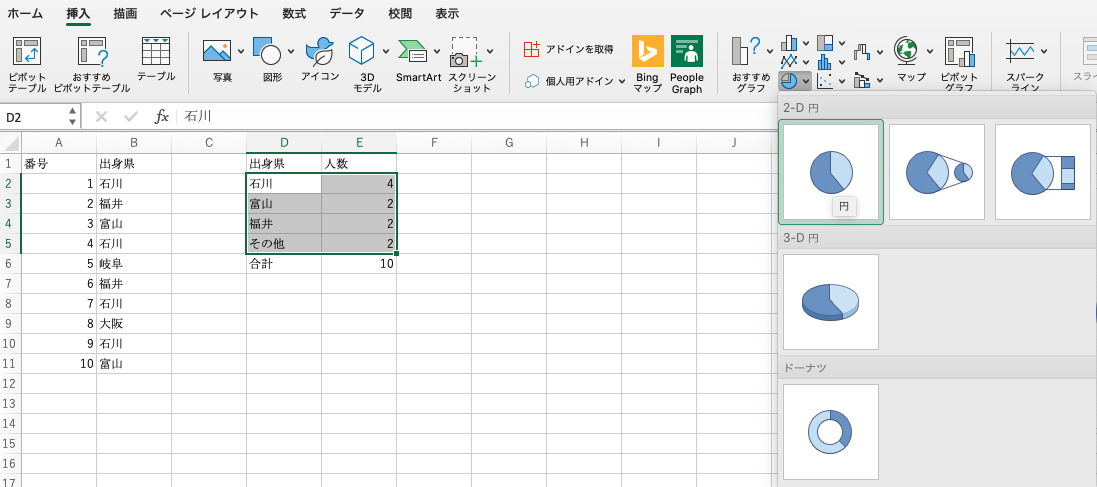
\includegraphics[width=6cm]{chap2/piechart_select_data.png}
        \caption{データを選択した状態}
        \label{fig:piechart_select_data}
    \end{minipage}
\end{figure}
\begin{figure}[tb]
    \begin{minipage}{0.5\hsize}
        \centering
        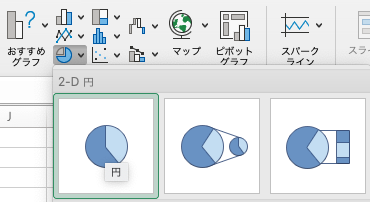
\includegraphics[width=5cm]{chap2/piechart_menu.png}
        \caption{リボン内の円グラフのアイコン}
        \label{fig:piechart_menu}
    \end{minipage}
    \begin{minipage}{0.5\hsize}
        \centering
        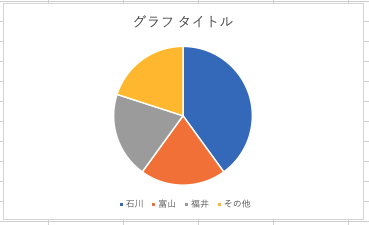
\includegraphics[width=6cm]{chap2/piechart_plain.png}
        \caption{できた円グラフ}
        \label{fig:piechart_plain}
    \end{minipage}
\end{figure}
\begin{figure}[tb]
    \begin{minipage}{0.5\hsize}
        \centering
        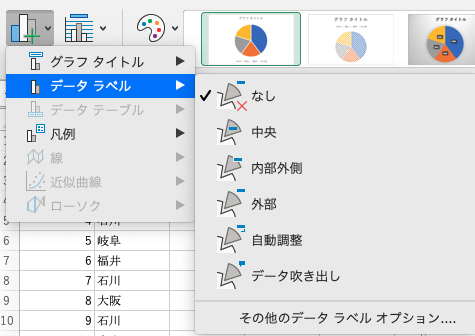
\includegraphics[width=5cm]{chap2/piechart_label_menu.png}
        \caption{リボン内のラベルメニュー}
        \label{fig:piechart_label_menu}
    \end{minipage}
    \begin{minipage}{0.5\hsize}
        \centering
        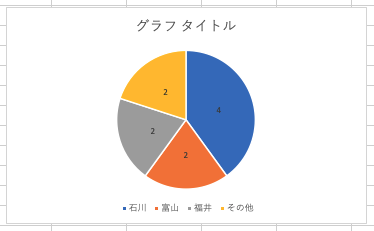
\includegraphics[width=6cm]{chap2/piechart_labeled.png}
        \caption{人数が記入された円グラフ}
        \label{fig:piechart_labeled}
    \end{minipage}
\end{figure}

\begin{figure}[tb]
    \begin{minipage}{0.5\hsize}
        \centering
        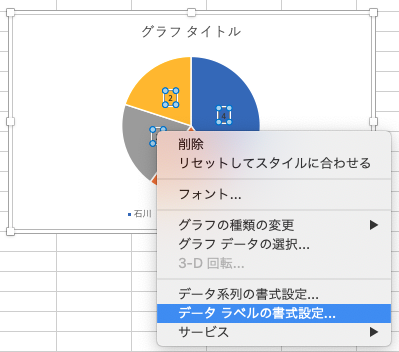
\includegraphics[width=5cm]{chap2/piechart_select_label_option.png}
        \caption{ラベルの書式設定を選ぶ}
        \label{fig:piechart_select_label_option}
    \end{minipage}
    \begin{minipage}{0.5\hsize}
        \centering
        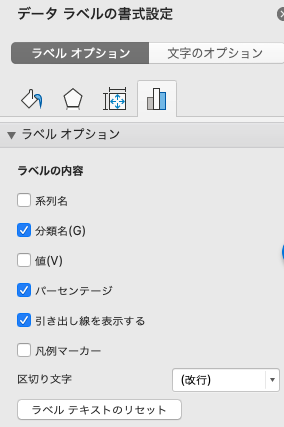
\includegraphics[width=6cm]{chap2/piechart_label_option.png}
        \caption{ラベルの書式設定}
        \label{fig:piechart_label_option}
    \end{minipage}
\end{figure}


\subsection{散布図}

\paragraph{散布図とは}

データの値同士の関係性を知りたいときがあります.
散布図は値の関係性を見るために用いられます.
例として,前回の演習で用いたアヤメのがく片の長さと幅 (iris.csv) の散布図(図\ref{fig:scatter})を示します.
散布図では関係を見るデータ,例ではアヤメのがく片の長さと幅をそれぞれ軸とします.
そして,データの組み合わせ,例ではアヤメのがく片の長さと幅の組み合わせを点で表します.
例の散布図を見ると,がく片の長さが長いほど幅が太くなる傾向がありそうなことが分かります.
データそれぞれ無関係な場合は,点は垂直,水平,円に分布します.

\begin{figure}[htbp]
    \centering
    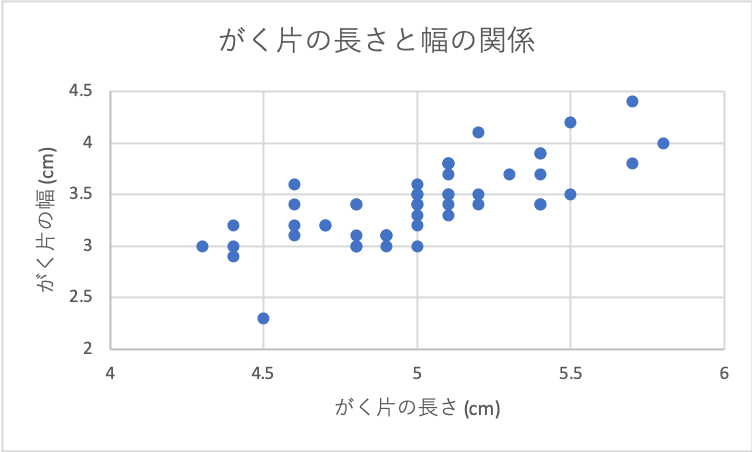
\includegraphics[width=8cm]{chap2/scatter.png}
    \caption{散布図}
    \label{fig:scatter}
\end{figure}

\paragraph{散布図の作成}

散布図も他のグラフの書き方と同じですが,データの列を2つ選ぶ点が異なります.

\begin{enumerate}
    \item データを開きます.今回は,アヤメデータiris.csvを用います.
    \item 散布図にしたいデータを選びます (図\ref{fig:scatter_data}).
    \item リボンの挿入を押します.
    そして,リボンにある散布図アイコンを押し,図\ref{fig:scatter_menu}に示す散布図ボタンを押します.
    そうすると図\ref{fig:scatter1}のような散布図が出来上がります.
    \item 作成した散布図はグラフの右上にデータ点が偏っています.
    グラフ全体にデータ点を広げるために,軸の値を調整します.
    はじめに縦軸を変更します (横軸から変更しても良いです).
    \begin{enumerate}
        \item 縦軸をクリックし (選び),右クリックを押して出てくる軸の書式 (図\ref{fig:scatter_axis}) を選びます.
        \item ウインドウの右端に出てくる軸の書式設定 (図\ref{fig:scatter_range}) の最小値,最大値を変更します.
        今回は最小値を2.0,最大値を4.5とします.
        同様に,横軸の最小値を4.0,最大値を6.0とします.
        そうすると図\ref{fig:scatter2}のようになります.
    \end{enumerate}
    \item 以上の操作で散布図は作れますが,グラフとして少し格好が悪いです.
    グラフには軸が何をあらわすか分かるようにラベルを付けます.
    \begin{enumerate}
        \item 軸にラベルを追加するには,リボンのグラフのデザインをクリックします.
        \item そして,軸を追加したいグラフを選び,リボンのグラフ要素を追加をクリックします.
        \item 出てきたメニュー (図\ref{fig:scatter_label}) の軸ラベル第1縦軸を選びます.
        そうすると,縦軸に``軸ラベル''というラベルが追加されます.
        \item ``軸ラベル''をクリックし選んだあと,更にクリックすると編集できるようになります.
        縦軸は``がく片の幅 (cm)''にしましょう\footnote{軸には単位を付けましょう.}.
        同様の手順でよく軸を``がく片の長さ (cm)''しましょう.
        そうすると,図\ref{fig:scatter3}のようなグラフができます.
    \end{enumerate}
    \item 必ずしもグラフにタイトル付ける必要はありませんが,今回はタイトルを付けます.
    ``グラフ タイトル''をクリックし選んだあと,更にクリックすると編集できるようになります.
    その状態で,``がく片の長さと幅の関係''に変更しましょう.
    以上の操作で,図\ref{fig:scatter}のようなグラフになります.
\end{enumerate}


\begin{figure}[tb]
    \begin{minipage}{0.5\hsize}
        \centering
        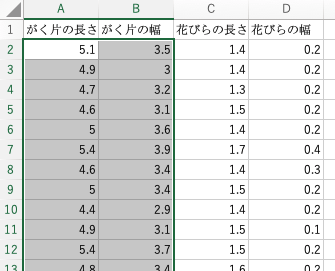
\includegraphics[width=5cm]{chap2/scatter_data.png}
        \caption{セルを選択した状態}
        \label{fig:scatter_data}
    \end{minipage}
 \begin{minipage}{0.5\hsize}
        \centering
        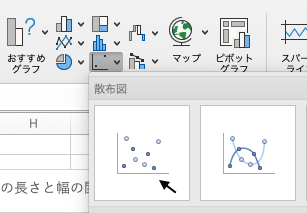
\includegraphics[width=6cm]{chap2/scatter_menu.png}
        \caption{散布図を選択する}
        \label{fig:scatter_menu}
    \end{minipage}
    \\
    \begin{minipage}{0.5\hsize}
        \centering
        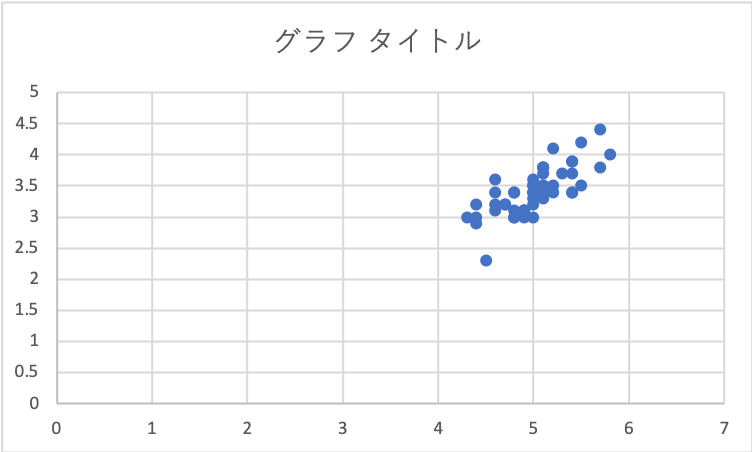
\includegraphics[width=6cm]{chap2/scatter1.png}
        \caption{未完成な散布図}
        \label{fig:scatter1}
    \end{minipage}
    \begin{minipage}{0.5\hsize}
        \centering
        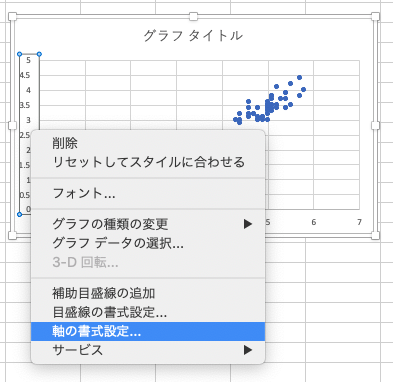
\includegraphics[width=4cm]{chap2/scatter_axis.png}
        \caption{軸のメニュー}
        \label{fig:scatter_axis}
    \end{minipage}
\end{figure}

\begin{figure}[tb]
    \begin{minipage}{0.5\hsize}
        \centering
        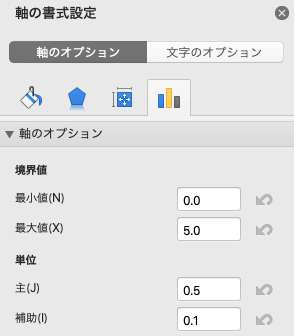
\includegraphics[width=4cm]{chap2/scatter_range.png}
        \caption{軸の範囲の設定}
        \label{fig:scatter_range}
    \end{minipage}
    \begin{minipage}{0.5\hsize}
        \centering
        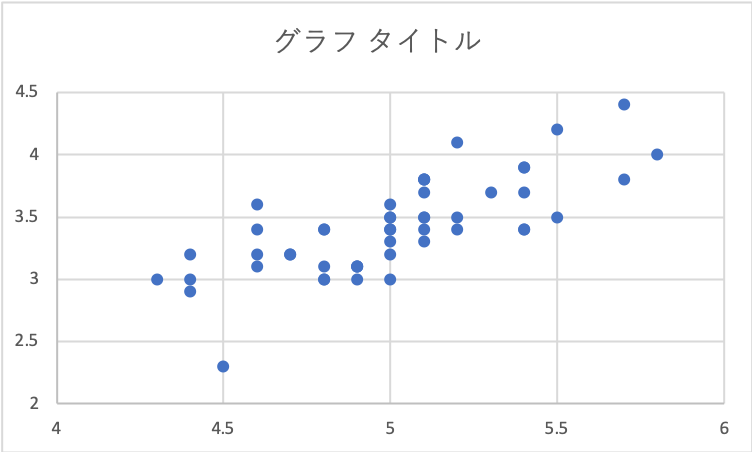
\includegraphics[width=6cm]{chap2/scatter2.png}
        \caption{軸の範囲を変えた散布図}
        \label{fig:scatter2}
    \end{minipage}
\end{figure}

\begin{figure}[tb]
    \begin{minipage}{0.5\hsize}
        \centering
        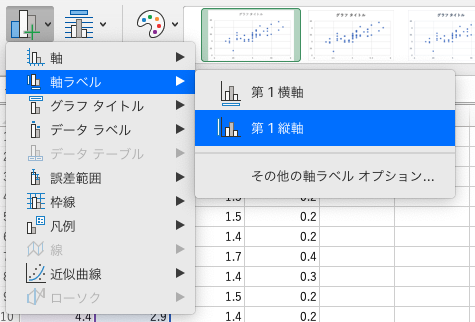
\includegraphics[width=5cm]{chap2/scatter_label.png}
        \caption{軸の範囲の設定}
        \label{fig:scatter_label}
    \end{minipage}
    \begin{minipage}{0.5\hsize}
        \centering
        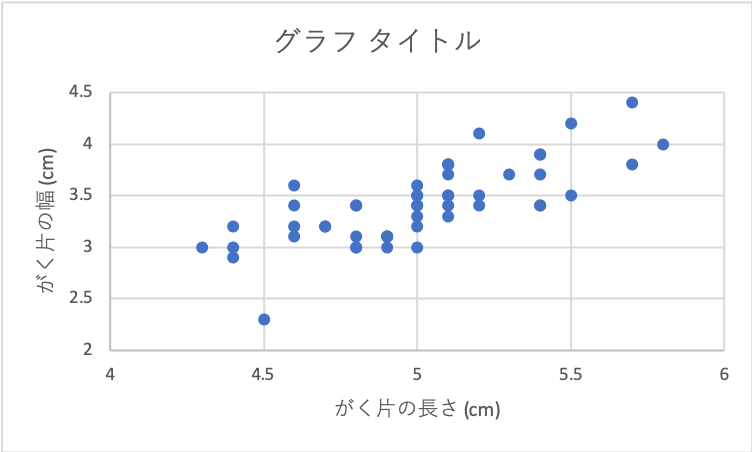
\includegraphics[width=6cm]{chap2/scatter3.png}
        \caption{軸のラベルを付けた散布図}
        \label{fig:scatter3}
    \end{minipage}
\end{figure}


\section{相関係数}

\paragraph{相関係数とは}

散布図では,視覚的に2つのデータの関係性を見ることができます.
しかし,図ではそのデータがどの程度関係しているのか定量的に分かりません.
定量的に2つのデータの関係を見る場合は相関係数を用います.
相関係数は次の式で計算されます.
\begin{equation}
    \label{eq:1}
    r = \frac{\frac{1}{N} \sum_{i=1}^N (x_i - \bar{x})(y_i - \bar{y})}{\sqrt{\frac{1}{N} \sum_{i=1}^N (x_i - \bar{x})^2} \sqrt{\frac{1}{N} \sum_{i=1}^N(y_i - \bar{y})^2}}
\end{equation}
相関係数はデータ同士が直線的な関係かどうかをみることができます.
相関係数が正の場合は正の相関,負の場合を負の相関と言います.
正の相関の場合,一方のデータの値が増えれば,もう一方のデータの値も増えるという関係があることが分かります.
負の相関の場合,一方のデータの値が増えれば,もう一方のデータの値は減るという関係があることが分かります.
しかし,U字型であったりS字型の関係であった場合は相関係数ではその関係性を定量化することはできません.


\paragraph{相関係数の計算}

Excelで相関係数を求めるのは簡単です.前回の総和を求めたのと同じ要領で行います.しかし,今回は2列データがありますので,そこだけ注意しましょう.

\begin{enumerate}
    \item データを開きます.今回も先程用いたアヤメデータiris.csvを用います.
    \item 相関係数を入れるセルを選択します.
    \item ``=CORREL(''と入力します.
    \item 相関係数を求めたいデータの列を2つ選びます.
    \item ``)''と入力します.そうすると,相関係数が表示されます.
\end{enumerate}

\section{回帰直線}

\paragraph{回帰直線とは}

2つデータの値同士の関係を知るために散布図を用いる事ができることを先程述べました.
図\ref{fig:regression}のように,その関係性を直線で表したものを回帰直線と言います.
回帰直線は,データの分布を直線に近似したものです.
もう少し簡単に言えば,2つのデータの関係を直線の式$y=ax+b$に強制的に表したものです\footnote{直線近似の方法は,この講義の範疇を超えているので説明しません.興味がある人は調べてみましょう.}.

\begin{figure}[htbp]
    \centering
    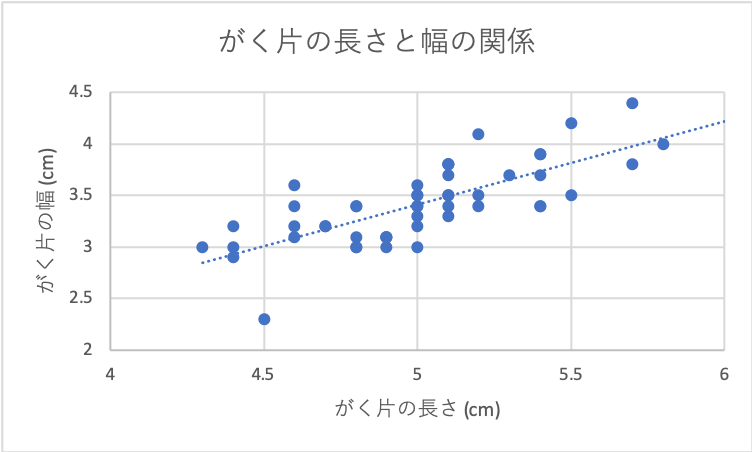
\includegraphics[width=6cm]{chap2/regression.png}
    \caption{散布図と回帰直線}
    \label{fig:regression}
\end{figure}

\paragraph{回帰直線の作成}

先程作成した散布図に回帰直線を追加します.

\begin{enumerate}
    \item 回帰直線を追加したい散布図を選びます.今回は,先ほど作成したアヤメデータの散布図に回帰直線を追加します.
    \item リボンの``グラフのデザイン''を選びます.
    \item 図\ref{fig:regression_menu}のように,近似曲線の線形予測を選びます.
    そうすると,図\ref{fig:regression}のような回帰直線がかかれます.
    軸の範囲が変わった場合は,見やすいように変更しましょう.
\end{enumerate}

\begin{figure}[htbp]
    \centering
    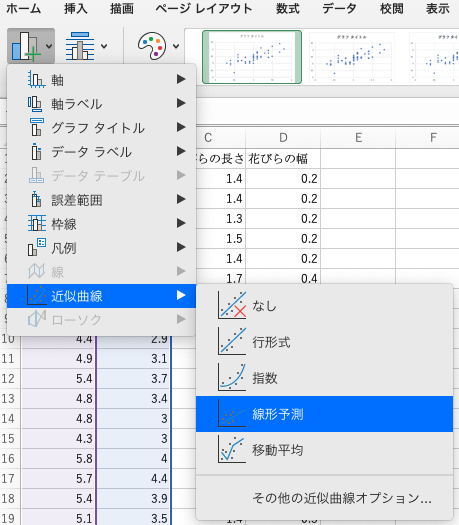
\includegraphics[width=6cm]{chap2/regression_menu.png}
    \caption{散布図}
    \label{fig:regression_menu}
\end{figure}

\section{演習}

\practice
temp\_city.csvファイルから棒グラフを作りなさい.ただし,横軸は都市,縦軸は気温(度)にしなさい.

\practice
2019年4月8日の小松市の気温データtemp.csvから折れ線グラフを作りなさい.ただし,横軸は時間(時),縦軸は気温(度)にしなさい.

\practice
2020年4月21日までの石川県内のコロナウイルス感染者情報COVID-19\_Ishikawa.csv\footnote{SIGNATEのCOVID-19 Challengeで作成されているデータを用いました.https://signate.jp/competitions/261}から,感染者の男女の割合を円グラフで表しなさい.

\practice
私鉄の資本金と従業員数のデータshitetsu.csvから散布図をかきなさい.ただし,横軸は資本金,縦軸は従業員数にしなさい
\footnote{http://www.qmss-matsubara.sakura.ne.jp/databank/index.htmlの私鉄データを用いました.}.

\practice
私鉄の資本金と従業員数のデータshitetsu.csv内の資本金と従業員数の相関係数を求めなさい.

\practice
演習4で作成した散布図に回帰直線加えたものを作成しなさい.

\section{レポート提出}

レポートはreport2.docxの空欄を埋める形で作成し,kazuhisa.fujita@komatsu-u.ac.jpへ電子データで提出してください.データ形式はdocxもしくはpdfでお願いします.レポートの提出期限は次回の講義日までとします.
